% gc-10-Hyperbolic.tex

\documentclass[xcolor=dvipsnames]{beamer}
\usepackage{teachbeamer}

\title{Transcendental Functions and Differentials}
\subtitle{{\CourseNumber}, BCIT}

\author{\CourseName}

\date{February 23, 2018}

% \begin{figure}[h]
% 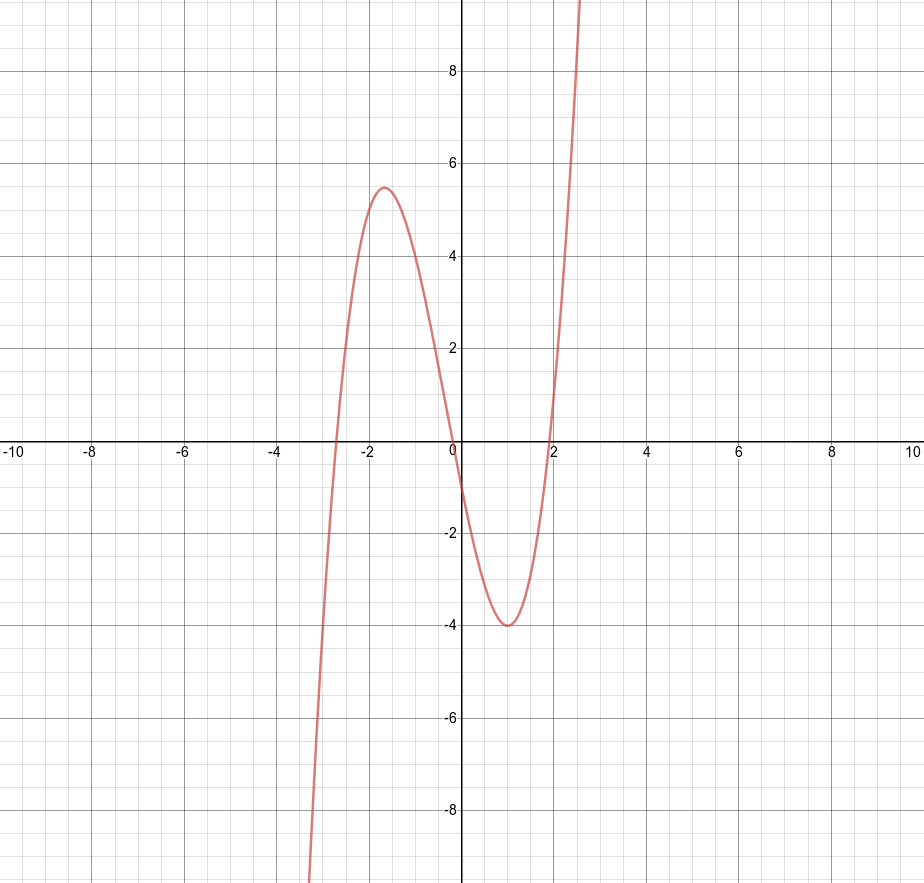
\includegraphics[scale=.3]{./diagrams/extrema1.png}
% \end{figure}

\begin{document}

\begin{frame}
  \titlepage
\end{frame}

\begin{frame}
  \frametitle{Linear Approximation I}
It would be tricky to calculate $\sqrt{3.92}$ by hand. Here is a way
to approximate this number. Let
\begin{equation}
  \label{eq:eiyahqui}
  f(x)=\sqrt{x}
\end{equation}
Then 
\begin{equation}
  \label{eq:geimaimo}
  f'(x)=\frac{1}{2\sqrt{x}}
\end{equation}
and the tangent line at $P=(4,2)$ is
\begin{equation}
  \label{eq:oocahpoh}
y=\frac{1}{4}x+1  
\end{equation}
% \begin{figure}[h]
% 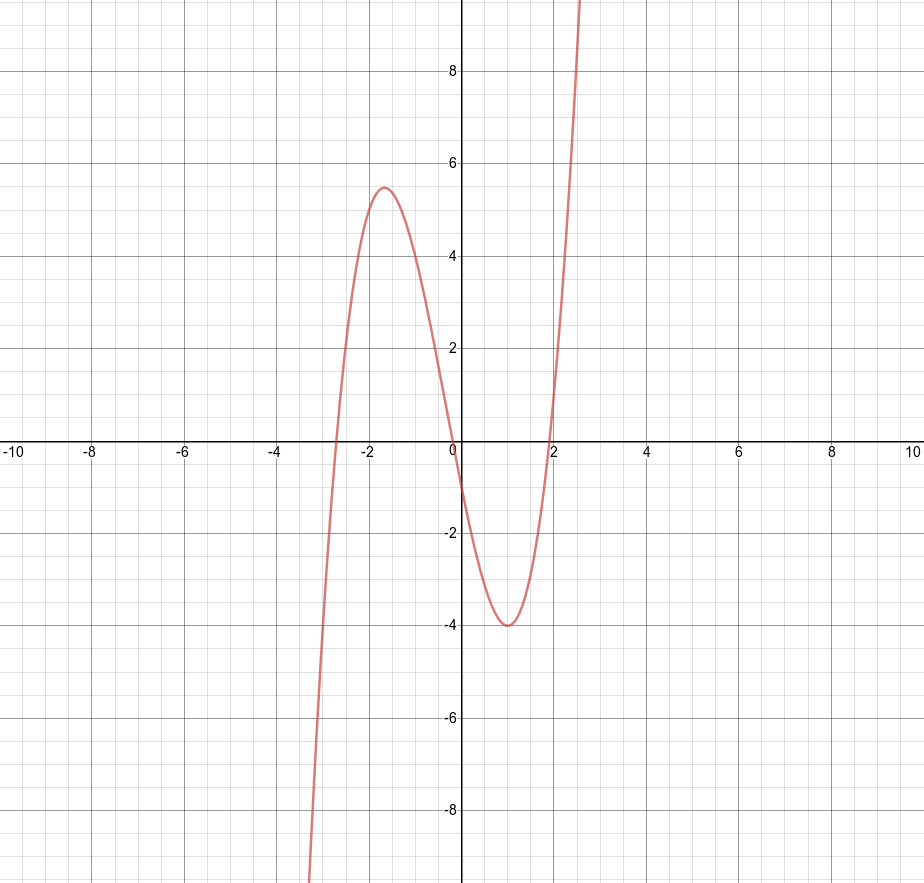
\includegraphics[scale=.3]{./diagrams/extrema1.png}
% \end{figure}
\end{frame}

\begin{frame}
  \frametitle{Linear Approximation II}
\begin{figure}[h]
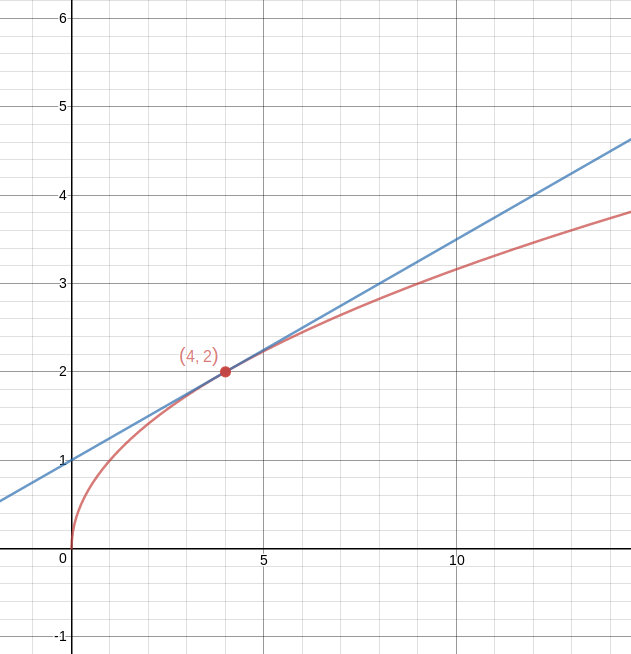
\includegraphics[scale=.25]{./diagrams/linapp1.png}
\end{figure}
Let's use how close the function is to the tangent line around the point $P=(4,2)$ to approximate $\sqrt{3.92}$.
\begin{equation}
  \label{eq:chairaey}
  1.9799=\sqrt{3.92}=f(3.92)\approx{}\frac{1}{4}\cdot{}3.92+1=1.98
\end{equation}
% Pretty good approximation!
\end{frame}

\begin{frame}
  \frametitle{Differentials}
It will be useful to define an independent variable $dx$ called a
\alert{differential}. The variable $dy$ is dependent on $dx$ and $x$.
It is determined by
\begin{equation}
  \label{eq:ahngieng}
  dy=f'(x)dx
\end{equation}
Now have a look at
\begin{equation}
  \label{eq:uzeepahv}
  f(x+dx)\approx{}f'(x)(x+dx)+f(x)-f'(x)x=\notag
\end{equation}
\begin{equation}
  \label{eq:ahghuako}
  f(x)+f'(x)dx=f(x)+dy
\end{equation}
This is the linear approximation we were talking about. 
\end{frame}

\begin{frame}
  \frametitle{Differentials}
\begin{figure}[h]
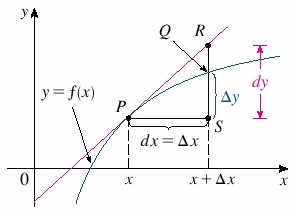
\includegraphics[scale=3]{./diagrams/differentials.jpg}
\end{figure}
\end{frame}

\begin{frame}
  \frametitle{Measurement Error}
Differentials are often used to approximate measurement errors. 

\bigskip

\beispiel{Volume of a Sphere}\label{ex:ootiteij} The radius of a
sphere was measured and found to be 21 cm with a possible error in
measurement of at most 0.05 cm. What is the maximum error in using
this value of the radius to compute the volume of the sphere?

\bigskip

If $V(r)=(4/3)r^{3}\pi$, then the answer to this question can be
approximated using (where $dr=\Delta{}r$ is the measurement error)
\begin{equation}
  \label{eq:faeshiur}
  dV=V'(r)dr
\end{equation}
The precise answer is often called $\Delta{}V$, which is approximated
by $dV$.
\end{frame}

\begin{frame}
  \frametitle{Differentials Exercises I}
{\ubung} Find the linearization $L(x)$ of the function at $a$ and
use it to approximate the function value at $b$.
\begin{enumerate}
\item $\displaystyle f(x)=x^{4}+3x^{2},a=-1,b=-0.923$
\item $\displaystyle f(x)=\ln{}x,a=1,b=1.1$
\item $\displaystyle f(x)=\cos{}x,a=\pi/2,b=82^{\circ}$
\item $\displaystyle f(x)=x^{\frac{3}{4}},a=16,b=16.3$
\end{enumerate}
\end{frame}

\begin{frame}
  \frametitle{Differentials Exercises II}
{\ubung} Find the linear approximation of the function 
\begin{equation}
  \label{eq:ceengaet}
g(x)=\sqrt[3]{1+x}
\end{equation}
at $a=0$ and use it to approximate the numbers 
\begin{equation}
  \label{eq:ciaghier}
\sqrt[3]{0.95}
\end{equation}
and
\begin{equation}
  \label{eq:woozahme}
\sqrt[3]{1.1}
\end{equation}
\end{frame}

\begin{frame}
  \frametitle{Differentials Exercises III}
{\ubung} Find the differential of each function.
\begin{enumerate}
\item $\displaystyle y=x^{2}\sin{}2x$ 
\item $\displaystyle y=\ln\sqrt{1+t^{2}}$
\item $\displaystyle y=e^{-u}\cos{}u$
\item $\displaystyle y=e^{\tan\pi{}t}$
\end{enumerate}
\end{frame}

\begin{frame}
  \frametitle{Differentials Exercises IV}
{\ubung} The edge of a cube was found to be 30cm with a possible error
in measurement of 0.1cm. Use differentials to estimate the error in
computing the volume of the cube and the surface area of the cube.

\bigskip

{\ubung} Use differentials to estimate the amount of paint needed to
apply a coat of paint 0.05cm thick to a hemisphere dome with diameter
50m.
\end{frame}

\begin{frame}
  \frametitle{Transcendental Functions}
Let's say that (among others) there are two extended families of
functions. On the one hand, there are \alert{polynomials} and their
relatives. Constant functions, the identity function, linear
functions, and polynomial functions with degrees greater or equal to
two are polynomial functions. Rational functions are not polynomial
functions, but they belong to the extended family. Functions with root
signs also are not polynomial functions, but they belong to the
extended family.

\bigskip

On the other hand, there are \alert{exponential functions} and their
relatives. Logarithmic functions are not exponential functions, but
they belong to the extended family as the inverse of the exponential
function. Where do trigonometric functions belong?
\end{frame}

\begin{frame}
  \frametitle{Complex Algebra}
  In order to answer this question, it is useful to go on a field trip
  to the complex numbers. Complex numbers are numbers of the form
  $a+b\cdot{}i$, where $a$ and $b$ are real numbers and $i$ has the
  interesting property of $i^{2}=-1$, so $i$ is not a real number.

\bigskip

Once you have done some complex algebra, it turns out that (Euler's formula)
\begin{equation}
  \label{eq:siquohjo}
  e^{ix}=\cos{}x+i\cdot{}\sin{}x  
\end{equation}
That means that
\begin{equation}
  \label{eq:oixiekae}
  \cos{}x=\frac{1}{2}\left(e^{ix}+e^{-ix}\right)
\end{equation}
\begin{equation}
  \label{eq:aurooshi}
  \sin{}x=\frac{1}{2i}\left(e^{ix}-e^{-ix}\right)
\end{equation}
To show that this is true add or subtract Euler's formula for $x$ and $-x$.
\end{frame}

\begin{frame}
  \frametitle{Euler's Formula}
We haven't defined the sine and cosine function on the imaginary
numbers yet. Using Euler's formula, it makes sense to define
\begin{equation}
  \label{eq:xohzunei}
  \cos(iy)=\frac{1}{2}\left(e^{-y}+e^{y}\right)
\end{equation}
\begin{equation}
  \label{eq:eeghaefi}
  \sin(iy)=\frac{1}{2i}\left(e^{-y}-e^{y}\right)
\end{equation}
These look (almost) like plain old real-valued functions, and they
should have many of the special features of trigonometric functions
(think of all those identities!).
\end{frame}

\begin{frame}
  \frametitle{Hyperbolic Functions Definition}
Let's return to the safe ground of real-valued functions on the
domain of the real numbers. We define
\begin{equation}
  \label{eq:gomedaek}
  \cosh{}x=\frac{1}{2}\left(e^{x}+e^{-x}\right)
\end{equation}
\begin{equation}
  \label{eq:teeyavah}
  \sinh{}x=\frac{1}{2}\left(e^{x}-e^{-x}\right)
\end{equation}
\begin{equation}
  \label{eq:oeyuzahc}
  \tanh{}x=\frac{\sinh{}x}{\cosh{}x}
\end{equation}
\begin{equation}
  \label{eq:ainguchu}
  \coth{}x=\frac{\cosh{}x}{\sinh{}x}
\end{equation}
\end{frame}

\begin{frame}
  \frametitle{Identities and Derivatives}
The following can be checked easily:
\begin{equation}
  \label{eq:wahquain}
  \cosh{}x+\sinh{}x=e^{x}\mbox{ (compare this to Euler's Formula)}
\end{equation}
\begin{equation}
  \label{eq:thaevuan}
  \cosh^{2}x-\sinh^{2}x=1
\end{equation}
\begin{equation}
  \label{eq:gahngoip}
  (\sinh{}x)'=\cosh{}x
\end{equation}
\begin{equation}
  \label{eq:shahsuuw}
  (\cosh{}x)'=\sinh{}x
\end{equation}
There is lots more, but this is enough theory for now. The take-home
lesson: once you expand the real numbers to the complex numbers,
trigonometric functions turn out to be exponential functions in disguise.
\end{frame}

\begin{frame}
  \frametitle{Unit Circles and Hyperbolas}
$\cosh(x)$ and $\sinh(x)$ are called \alert{hyperbolic} functions
because they parametrize the unit hyperbola $x^{2}-y^{2}=1 $ the way
$\cos(x)$ and $\sin(x)$ parametrize the unit circle $x^{2}+y^{2}=1$.
\begin{figure}[h]
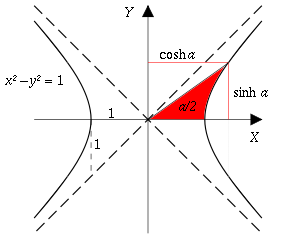
\includegraphics[scale=.5]{./diagrams/hyper.png}
\end{figure}
\end{frame}

\begin{frame}
  \frametitle{Catenaries and Ocean Waves}
  \beispiel{Catenaries} Have you ever wondered what function graph
  models a hanging wire? Galileo thought it was a parabola. It turns
  out to be $\cosh(x)$. The function
  \begin{equation}
    \label{eq:keechieg}
    f(x)=c+a\cosh\left(\frac{x}{a}\right)
  \end{equation}
  is called a \alert{catenary}.

  \bigskip

  \beispiel{Ocean Waves} Another application occurs in the description
  of ocean waves. The velocity of a water wave with length $L$ moving
  across a body of water with depth $d$ is modeled by the function
  ($g\approx{}9.8m/s^{2}$)
  \begin{equation}
    \label{eq:oghaivae}
    v=\sqrt{\frac{gL}{2\pi}\tanh\left(\frac{2\pi{}d}{L}\right)}
  \end{equation}
\end{frame}

\begin{frame}
  \frametitle{The USS Ramapo in Mountainous Waves}
  \beispiel{USS Ramapo} In February, 1933, the USS Ramapo, a 146 meter
  (478 ft) Navy oiler found itself in an extraordinary storm on its
  way from Manila to San Diego. The storm lasted 7 days and stretched
  from the coast of Asia to New York, producing strong winds over
  thousands of miles of unobstructed ocean. Driven from behind by
  winds on the order of 60 knots, the crew had time to carefully
  observe the nearly sinusoidal mountainous waves. An officer on the
  deck observed the crest of the wave approaching from behind just
  over the level of the crow's nest while the stern of the ship was at
  the trough of the wave. Subsequent scaling yielded the height of 34
  meters for the wave.
\end{frame}

\begin{frame}
  \frametitle{The USS Ramapo in Mountainous Waves}
  {\ubung} How fast did the waves travel across the ocean if the depth
  of the ocean was 3000 metres?
\begin{figure}[h]
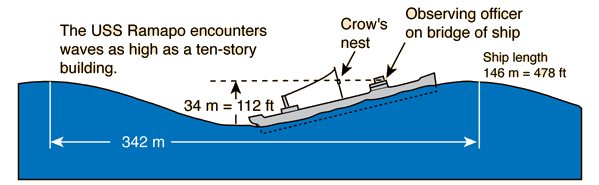
\includegraphics[scale=.5]{./diagrams/ramapo.png}
\end{figure}
The ship's crew measured the period of the waves at $14.8$ seconds.
Does this number agree with the velocity you calculated?

Notice that if you could measure the velocity of the waves you could
calculate the depth of the ocean using \alert{inverse hyperbolic
  functions}. 
\end{frame}

\begin{frame}
  \frametitle{Exercises}
{\ubung} Find the numerical value of $\tanh{}2$ and $\cosh(\ln{}3)$.

\medskip

{\ubung} Show that $\sinh(x)$ is an odd function and that $\cosh(x)$
is an even function.

\medskip

{\ubung} Prove the double angle formula
\begin{equation}
  \label{eq:chieshah}
  \cosh{}2x=\cosh^{2}x+\sinh^{2}x
\end{equation}
\end{frame}

\begin{frame}
  \frametitle{Exercises}
{\ubung} Differentiate
\begin{equation}
  \label{eq:sahwiesh}
  f(x)=\sinh(\cosh{}z)
\end{equation}
\begin{equation}
  \label{eq:gaitocee}
  g(y)=\cosh(\ln{}x)
\end{equation}
\begin{equation}
  \label{eq:pasaanee}
  h(z)=\tanh(1+e^{2x})
\end{equation}
\end{frame}

\begin{frame}
  \frametitle{Exercises}
  % solution: see gc-lec-20180302.pdf (graffiti) page 1
  % this is a nice segue to inverse hyperbolic trig functions
{\ubung} At what point of the curve
\begin{equation}
  \label{eq:geipaifo}
  y=\cosh{}x
\end{equation}
does the tangent have slope 1?
\end{frame}

\begin{frame}
  \frametitle{Exercises}
{\ubung} 
% solution: see coshANDsec.html
Choose the correct answer for what follows from $x=\ln(\sec\vartheta+\tan\vartheta)$:
\begin{enumerate}
\item $\cosh{}x=\sin\vartheta$
\item $\cosh{}x=\cos\vartheta$
\item $\cosh{}x=\csc\vartheta$
\item $\cosh{}x=\sec\vartheta$
\end{enumerate}
\end{frame}

\begin{frame}
  \frametitle{Exercises}
{\ubung} Evaluate
\begin{equation}
  \label{eq:ielaicah}
  \lim_{x\rightarrow\infty}\frac{\sinh{}x}{e^{x}}
\end{equation}
\end{frame}

\begin{frame}
  \frametitle{Exercises}
{\ubung} A telephone line hangs between two poles 14 metres apart in
the shape of a catenary
\begin{equation}
  \label{eq:lufaebeg}
  y=20\cosh\left(\frac{x}{20}\right)-15
\end{equation}
where $x$ and $y$ are measured in metres. Find the slope of this curve
where it meets the right pole in order to determine the angle between
the line and the pole.
\end{frame}

\begin{frame}
  \frametitle{Exercises}
{\ubung} If you know that the depth of the ocean is 1500 metres and
you measure the length $L$ of a wave to be 17 metres with a 50cm
margin of error, then what is your margin of error for the calculated
velocity of the wave? Use equation (\ref{eq:oghaivae}).
\end{frame}

\begin{frame}
  \frametitle{End of Lesson}
Next Lesson: Newton's Method and Optimization
\end{frame}

\end{document}

